\documentclass[AutoFakeBold,AutoFakeSlant]{beamer}

\usepackage[british]{babel}
\usepackage{graphicx,hyperref,sysu,url}
\usepackage{ctex}
\usepackage{booktabs}
\usepackage{tabularx}
\usepackage{multirow}
\usepackage[ruled,linesnumbered]{algorithm2e}
\usepackage{color}
\usepackage{amsmath,bm}
\usepackage{lmodern}
\usepackage{utopia}
\usepackage{amsfonts}
\usepackage{amsthm}
\usepackage{amssymb}

\definecolor{sysugreen}{RGB}{0,88,38}
\definecolor{sysugreendark}{RGB}{5,71,25}

\newcommand{\ctoday}{\number\year 年 \number\month 月 \number\day 日}

\setCJKmainfont[ItalicFont={SimSun}]{SimSun}
\setCJKsansfont{SimHei}
\setCJKmonofont{FangSong}

\RequirePackage{fontspec,xltxtra,xunicode}
\setmainfont[Mapping=tex-text]{Times New Roman}
\setsansfont[Mapping=tex-text]{Arial}
\setmonofont{Consolas}
\usefonttheme[onlymath]{serif}

\bibliographystyle{IEEETran}

\title[多模态文档问答系统期末展示]{基于强化学习决策的文档理解与检索多模态问答系统}
\author[刘天翔\quad 杨毅涵\quad 郭翊涛]{
  刘天翔\quad 杨毅涵\quad 郭翊涛
  \texorpdfstring{\\\medskip {\small 计算机科学与技术}}{}
}
\institute[Sun Yat-Sen University]{中山大学计算机学院}
\date[\today]{\ctoday}

\begin{document}

% 作者信息
\author[刘天翔\quad 杨毅涵\quad  郭翊涛]{
  刘天翔\quad 杨毅涵\quad  郭翊涛 
  \texorpdfstring{\\\medskip {\small 计算机科学与技术}}{}
}

\begin{frame}
  % 标题页
  \titlepage
\end{frame}
% 标题页不编号
\setcounter{framenumber}{0}

\begin{frame}
  % 目录页
  \frametitle{目\quad 录}
  % 双栏
  % \begin{multicols}{2}
  %   \tableofcontents
  % \end{multicols}
  \tableofcontents[hideallsubsections]
\end{frame}

\section{系统介绍}

\begin{frame}
  \frametitle{系统介绍：多模态文档问答助手}
  \small
  \begin{itemize}
    \item 本项目旨在构建一个集文档解析、视觉定位、检索增强生成和自然语言理解于一体的多模态文档智能问答系统。
    \item 系统面向 PDF、图片等非结构化文档，识别其中的文本、表格、公式、图表和局部视觉区域，并通过多模态 RAG 实现长文档精准检索与结构化问答。
    \item 传统纯文本 RAG 往往把文档转成线性文本，面对图表数值、表格行列关系、广告标签、票据版面和局部视觉信息时，容易丢失页面结构和视觉语义。
    \item 因此，本系统围绕“文档解析-多模态证据检索-GRPO 决策模型-生成回答-PDF 高亮溯源”构建完整流程。
    \item 核心任务包括：多模态 RAG 架构构建、模型选择与自动决策、可解释性溯源。
  \end{itemize}
\end{frame}

\section{相关技术与系统架构}

\begin{frame}
  \frametitle{系统架构图}
  \begin{figure}[htbp]
    \centering
    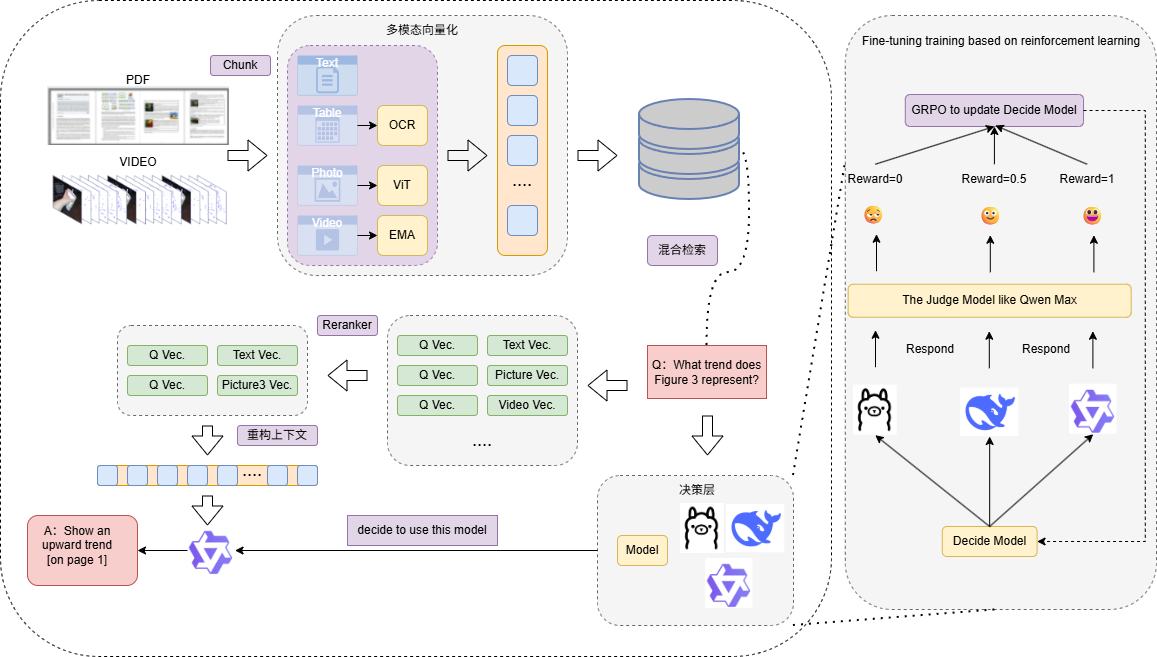
\includegraphics[width=0.92\textwidth]{image/frame.png}
  \end{figure}
\end{frame}


\begin{frame}
  \frametitle{多模态 Embedding 与 Fusion 实现}
  \begin{itemize}
    \item 系统先把页面解析结果统一整理为 evidence 对象，不把文本、表格和图像割裂成三个互不相关的库。
    \item 文本 chunk、OCR 文本和表格 Markdown 使用 BGE-M3 生成向量表示，作为文档问答中的基础文本 embedder。
    \item 表格区域先转换为 Markdown table，再参与向量化，使问题中的行名、列名、时间、数值和单位能与表格结构产生语义匹配。
    \item 图像侧使用轻量视觉特征或 Native ViT 图像编码器提取视觉向量，用于保留局部 crop、图表区域、页面截图和图片 chunk 的检索能力。
    \item 每条 evidence 同时绑定文本内容、页码、bbox、页面图路径、局部 crop、source type 和 modality，便于后续检索、生成和前端溯源。
  \end{itemize}
\end{frame}

\begin{frame}
  \frametitle{GRPO 决策模型实现}
  \begin{itemize}
    \item GRPO 模块的目标不是写死路由规则，而是训练一个 Decide Model，使其根据问题和候选 evidence 学会选择 LLM/VLM。
    \item Decide Model 接收用户问题、检索证据和问题类型信息，选择候选回答模型，例如文本 LLM、多模态 VLM 或图表增强 VLM。
    \item 候选模型基于同一问题和证据分别生成回答：普通文本题更适合文本 LLM，图表、票据、广告和局部页面区域题更依赖 VLM。
    \item Judge Model（如 Qwen-Max）根据答案正确性、证据一致性和完整性给出 reward，例如 0、0.5 或 1。
    \item 系统使用 GRPO 根据 reward 更新 Decide Model，使高分的模型选择在后续相似问题中更容易被采用。
  \end{itemize}
\end{frame}

\begin{frame}
  \frametitle{上下文重构、生成与前端溯源闭环}
  \small
  \begin{itemize}
    \item 生成阶段接收检索重排后的 evidence，以及 GRPO 决策模型输出的模型选择结果。
    \item 系统不会简单拼接 Top-K，而是按问题类型重构上下文：文本题保留高分文本 chunk，表格题加入 Markdown table，图表题加入页面标题、图表区域和局部 crop。
    \item 对票据、广告、商品标签等问题，系统优先保留字段名、品牌名、OCR anchor 和局部视觉区域，减少无关页面内容对 VLM 的干扰。
    \item 决策模型选出的 LLM/VLM 接收重构后的上下文进行回答；需要视觉理解的问题调用 Qwen3-VL-8B-Instruct。
    \item 输出结果时，模型给出答案和 evidence 编号；后端把 evidence id 映射回 page、chunk id、bbox、source type 和 image path。
    \item 前端接收答案、引用 evidence、页码和 bbox 后，在答案区展示引用，并根据页面缩放比例把 bbox 高亮到连续 PDF viewer 中。
  \end{itemize}
\end{frame}

\section{实验结果}

\begin{frame}
  \frametitle{实验表 1：Text-RAG 与 Our-RAG 性能对比}
  \scriptsize
  \resizebox{\textwidth}{!}{%
  \begin{tabular}{llrrrr}
    \toprule
    Dataset & Model & EM & ANLS & Answer Match & Avg. Latency(ms) \\
    \midrule
    DocVQA & Text-RAG & 0.5500 & 0.6230 & 0.6500 & 5697.80 \\
    DocVQA & Our-RAG & 0.9500 & 0.9620 & 0.9500 & 6124.35 \\
    ChartQA & Text-RAG & 0.2000 & 0.2300 & 0.2500 & 3451.81 \\
    ChartQA & Our-RAG & 0.8750 & 0.8960 & 0.9000 & 4896.42 \\
    Overall & Text-RAG & 0.3750 & 0.4265 & 0.4500 & 4574.81 \\
    Overall & Our-RAG & 0.9125 & 0.9290 & 0.9250 & 5510.39 \\
    \bottomrule
  \end{tabular}}
  \vspace{0.2cm}

  \begin{itemize}
    \item \textbf{总体性能}：Our-RAG 的整体 EM 达到 0.9125，ANLS 达到 0.9290，明显高于 Text-RAG。
    \item \textbf{DocVQA}：局部 crop 补充品牌、logo、票据版面和表格空间关系。
    \item \textbf{ChartQA}：chart region 使 VLM 能直接读取坐标轴、柱高、折线和数值比较关系。
    \item \textbf{效率表现}：优先传入问题相关的局部 crop，而不是整页多图输入。
  \end{itemize}
\end{frame}

\begin{frame}
  \frametitle{实验表 2：消融实验与错误分析}
  \scriptsize
  \resizebox{\textwidth}{!}{%
  \begin{tabular}{lrrrr}
    \toprule
    Model & EM & ANLS & Answer Match & Delta EM \\
    \midrule
    Our-RAG & 0.9125 & 0.9290 & 0.9250 & -- \\
    Our-RAG with Rule Decision & 0.9120 & 0.9280 & 0.9300 & -0.0005 \\
    Our-RAG without Reranker & 0.9030 & 0.9100 & 0.9120 & -0.0095 \\
    Our-RAG without Unified Embedding & 0.8950 & 0.9020 & 0.9000 & -0.0175 \\
    \bottomrule
  \end{tabular}}
  \vspace{0.25cm}

  \begin{itemize}
    \item Reranker 和统一多模态向量化是影响结果的关键因素。
    \item 错误主要来自复杂表格行列定位、局部视觉区域裁剪偏差、图表数值估读误差、生成答案格式波动。
  \end{itemize}
\end{frame}

\section{Demo 与反思}

\begin{frame}
  \frametitle{Demo 视频}
  \vspace{0.6cm}
  \begin{center}
    \fbox{\parbox{0.72\textwidth}{\centering\vspace{1.3cm}Demo 视频占位\vspace{1.3cm}}}
  \end{center}
\end{frame}

\begin{frame}
  \frametitle{反思：模型局限}
  \scriptsize
  \begin{itemize}
    \item \textbf{模块化系统而非端到端理解}：当前流程仍由 OCR、版面解析、统一 embedding、向量检索、Reranker、GRPO 决策和 VLM 生成串联组成，任何模块误差都会沿 pipeline 传播到最终回答。
    \item \textbf{证据质量依赖前置解析}：OCR 漏识别、表格结构抽取不完整或 figure/table/code 分类不准，会导致 evidence 缺失；在票据字段、广告标签、表格行列关系等问题上尤其明显。
    \item \textbf{空间定位仍有不稳定性}：系统保留页码、bbox 与页面图路径用于 PDF 高亮，但 bbox 偏移、局部 crop 过大或过小都会影响前端溯源效果，也会干扰 VLM 对关键区域的观察。
    \item \textbf{检索召回决定视觉输入上限}：如果向量检索和重排没有召回真正相关的 chunk 或页面区域，后续即使使用更强 VLM，也只能在错误或不完整上下文中生成答案。
    \item \textbf{复杂视觉推理仍受底层模型限制}：图表数值估读、隐含趋势比较、跨页表格、密集版面和多实体对应关系仍可能出现“证据定位正确但推理不充分”的情况。
    \item \textbf{长期任务能力不足}：系统能够完成当前文档、当前问题下的问答，但对跨文档持续记忆、多轮目标追踪、主动发现矛盾和长程任务规划的支持仍比较有限。
  \end{itemize}
\end{frame}

\begin{frame}
  \frametitle{展望：AGI 视角下的潜力与瓶颈}
  \scriptsize
  \begin{itemize}
    \item \textbf{文档智能是通向通用助手的重要入口}：真实知识并不只存在于纯文本中，还分布在 PDF、表格、图片、图表、扫描件和网页截图里，系统需要同时处理文本语义与视觉结构。
    \item \textbf{从“回答问题”走向“管理证据”}：接近 AGI 的文档系统不仅要能读懂内容，还要能定位来源、比较多个证据、判断冲突、解释推理过程，并把答案稳定溯源到原始文档。
    \item \textbf{本项目的可延展基础}：当前系统已经把多模态感知、检索增强、模型选择、局部视觉 crop、答案生成和 PDF 高亮连接起来，为后续加入更强的自我验证与交互反馈留下接口。
    \item \textbf{近期改进方向}：继续提升复杂版面解析、表格结构恢复、图表区域裁剪、答案格式规范化和 evidence 选择稳定性，降低 OCR 与 bbox 误差对最终结果的影响。
    \item \textbf{决策模型优化方向}：让 GRPO 决策模型积累更多真实问答轨迹和失败样本，根据问题类型、候选模型打分与证据质量动态选择 LLM/VLM、检索深度和视觉输入策略。
    \item \textbf{长期 AGI 瓶颈}：未来仍需要更强的多模态基础模型、跨文档长期记忆、任务规划、自我评估和持续学习能力，才能从“能回答文档问题的系统”进一步走向“能理解、使用并管理文档知识的智能体”。
  \end{itemize}
  \vspace{0.15cm}
  \begin{center}
    感谢老师与同学们的聆听。
  \end{center}
\end{frame}

\end{document}
